\section*{Results}

\begin{figure}[t]
  \centering
  \label{mov:trial1}
  \movie[externalviewer]{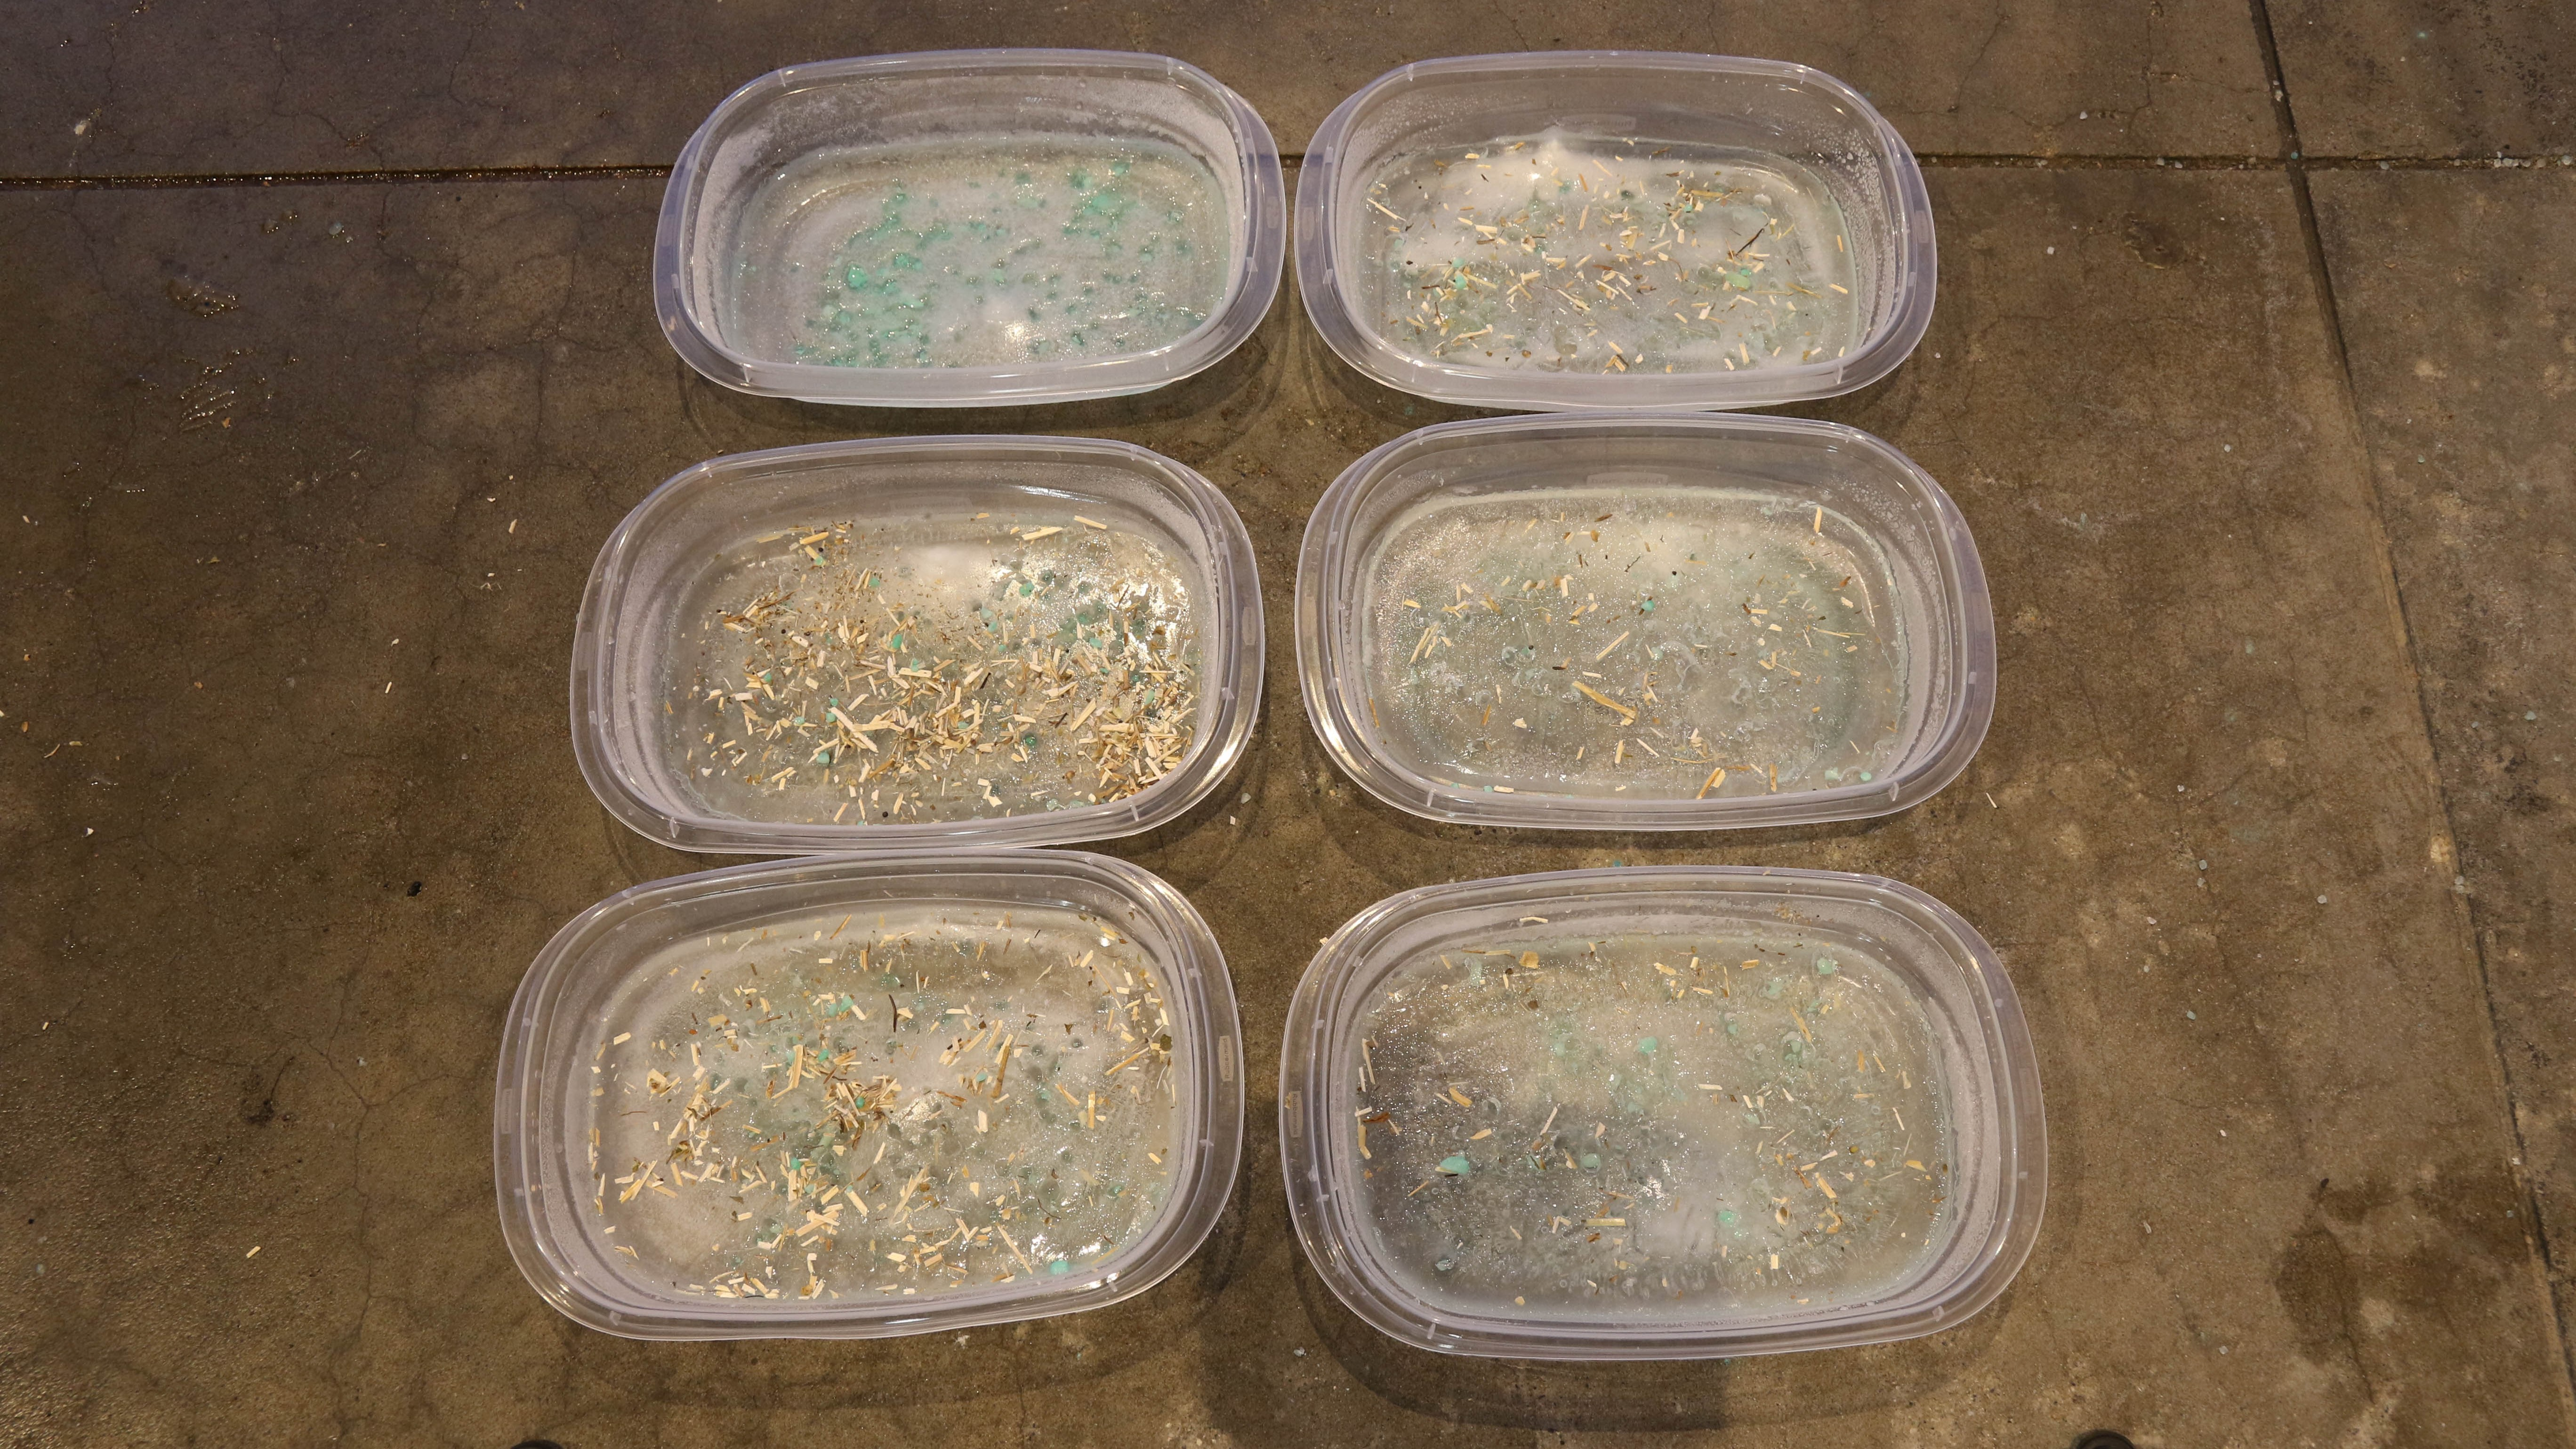
\includegraphics[width=\textwidth]{assets/icetest2-505.jpg}}{ice-timelapse1-compressed.mp4}
  \caption{\small Timelapse of trial 1. Samples are ordered 1--5 plus the control sample, from bottom to top on both columns, starting with the lowest rightmost column of containers. This video corresponds with the \texttt{ice-timelapse1-compressed.mp4} file provided with this report.}
\end{figure}
The first trial was performed in \SI{-8}{\degreeCelsius} weather.
Due to external circumstances, the trial could only be conducted for 60 minutes.
The timelapse can be viewed through \hyperref[mov:trial1]{Figure 1} as embedded multimedia.\footnote[1]{Adobe Acrobat Reader version 6 or later is \textbf{required} in order to play the timelapse through the PDF. By clicking the figure, Acrobat Reader will prompt to open the respective video file, to which the timelapse will play through the default video player on your system. Alternatively, you can view the video through the provided \texttt{.mp4} files.}
An additional small quantity of salt is added to each sample after 30 minutes because of lower effectiveness than expected.
The mixtures performed as expected of a deicing salt agent; all, to some degree, melted some of the ice and water could be seen accumulating at the bottom of the containers.
The control sample became notably porous within 15 minutes after applying the salt.
Once reaching the bottom of the container, the salt began to dissolve into the aforementioned water.
This resulted in the ice partially dislodging from the bottom of the container and was observed with the other samples in the trial.
All samples showed the same degree of increasing ice asperity in the duration of the experiment and demonstrated a degree of perforation from the salt.
Samples 1 and 2 were mildly perforated by the salt, undermined by latent refreezing after some time.
By contrast, sample 3--5 were moderately perforated and did not see any latent refreezing.
This is attributed to the absorption of the volume of hemp hurd, as it prevents the resulting water to refreeze.
While the control sample undoubtedly melted a greater volume of ice, the experimental samples showed a comparable amount of melting to a degree that is not insignificant.

\begin{figure}[t]
  \centering
  \label{mov:trial2}
  \movie[externalviewer]{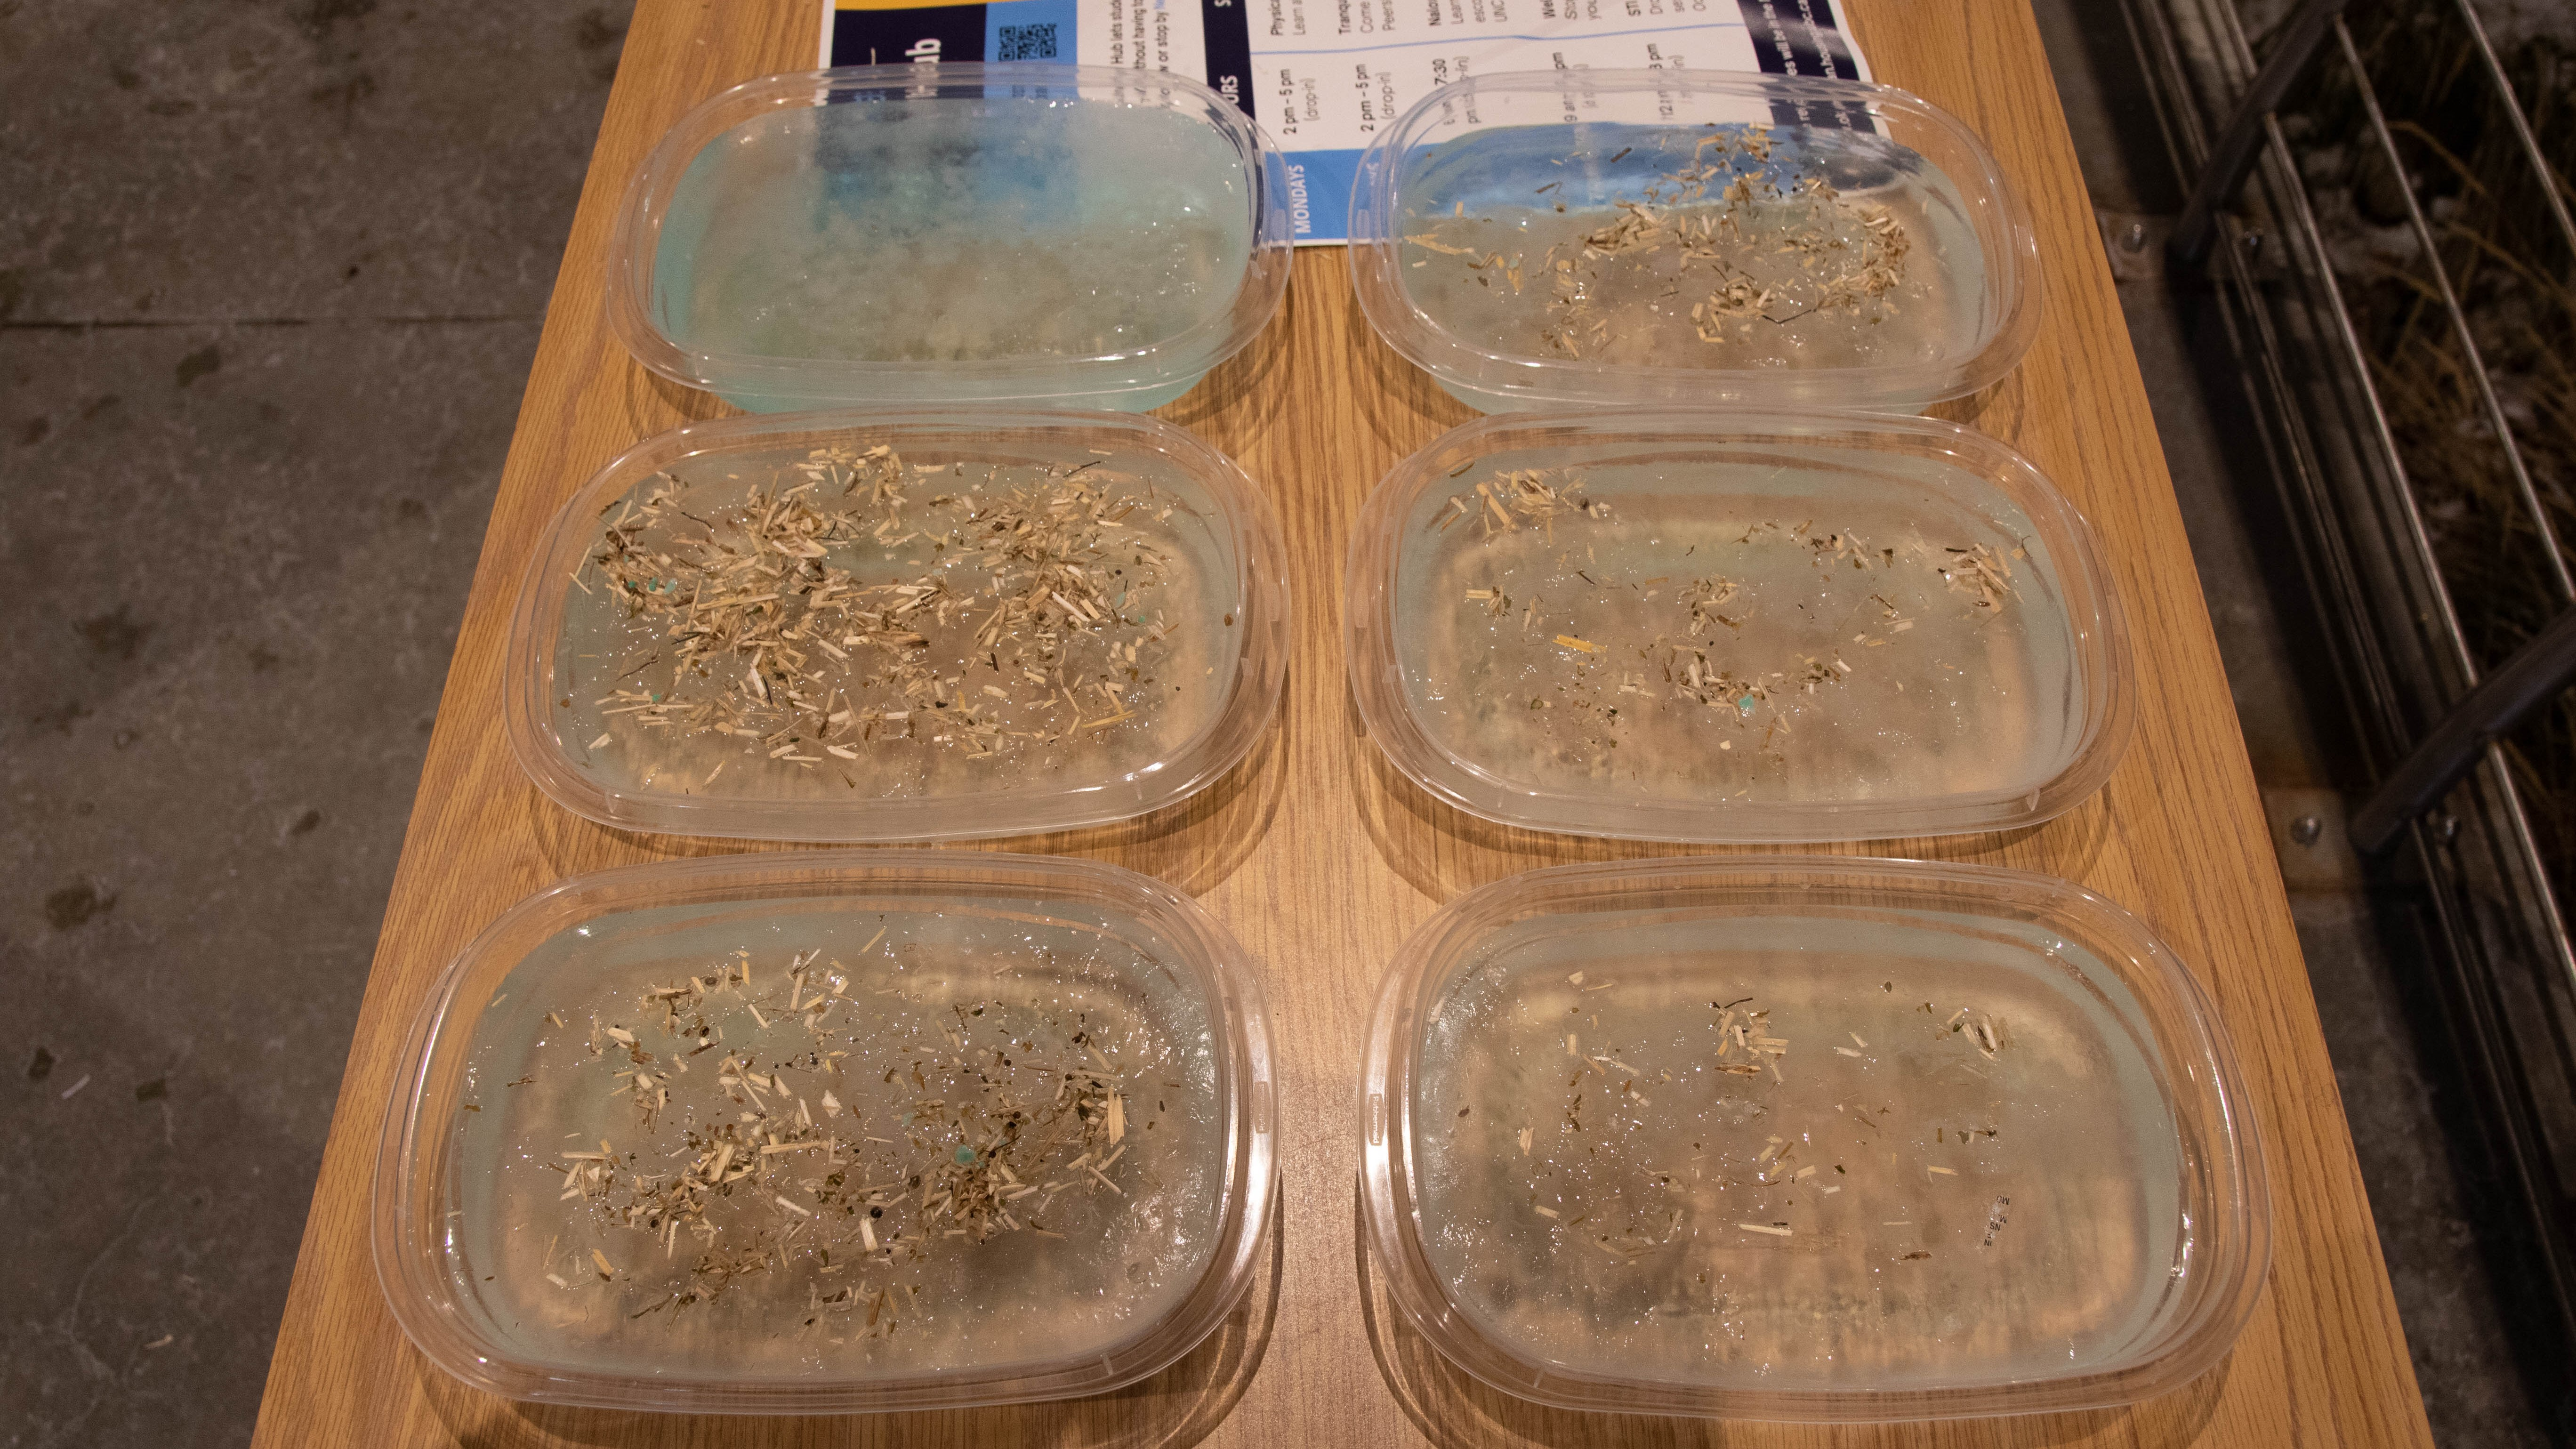
\includegraphics[width=\textwidth]{assets/icetest-800.jpg}}{ice-timelapse2-compressed.mp4}
  \caption{\small Timelapse of trial 2. Samples are ordered 1--5 plus the control sample, from bottom to top on both columns, starting with the lowest rightmost column of containers. This video corresponds with the \texttt{ice-timelapse2-compressed.mp4} file provided with this report.}
\end{figure}

The second trial was performed in \SI{-2}{\degreeCelsius} weather and conducted for 90 minutes.
Due to challenges in producing the ice for this trial, there was a significant amount of water \SI{5}{\mm} below the ice surface, a lesser thickness than what was originally intended for this trial.
The consequence resulted in the salt crystals completely dissolving after going through the \SI{5}{\mm} of ice.
The ice melted quicker than expected after application, likely due to the relatively warmer ambient temperature.
An additional small quantity of salt is added to each sample after 30 minutes because less ice was melted than expected.
Differences outstanding, the results were similar to the first trial.
Samples 1 and 2 showed some amounts of perforation and asperity, while 3--5 showed moderate amounts.
The control sample was heavily perforated and appeared likely to shatter with some pressure after 90 minutes had elapsed.
The perforation of the samples reduced the integrity of the ice, as found during the disposal of the samples.
Lastly, the hemp in all experimental samples seemed to infuse with the ice, becoming embedded in the surface.
